\documentclass[a4paper,12pt]{article}
\usepackage[papersize={216mm,330mm},tmargin=20mm,bmargin=20mm,lmargin=20mm,rmargin=20mm]{geometry}
\usepackage[english]{babel}
\usepackage[utf8]{inputenc}
\usepackage{amsmath,amssymb,mathabx}
\usepackage{lscape}
\usepackage{graphicx}
\usepackage{fancyhdr}
\usepackage{float}
\usepackage{listings} % For sexy code
\usepackage{xcolor} % For code highlighting
\usepackage{sourcecodepro} % changes default \ttfamily
\usepackage[T1]{fontenc} % need this for the font
\usepackage[font=normalsize,labelfont=bf]{caption} %For changing caption size

% Some colors for sexy code
\definecolor{codegreen}{rgb}{0,0.6,0}
\definecolor{codegray}{rgb}{0.5,0.5,0.5}
\definecolor{codepurple}{rgb}{0.58,0,0.82}
\definecolor{backcolour}{rgb}{1,1,1}

% listing custom propertie I confirm my intent to publish this project in the publicly accessible Overleaf Gallery. s
\lstset{
    language=C,                         % Set language to C
    basicstyle=\small\ttfamily,        % Smaller, readable font
    keywordstyle=\color{blue},          % Keyword font style
    commentstyle=\color{codegreen},     % Comment font style
    stringstyle=\color{codepurple},     % String font style
    showstringspaces=false,             % Do not underline spaces within strings
    breaklines=true,                    % Automatic line breaking
    tabsize=4,                          % Tab size
    numbers=left,                       % Line numbers on the left
    numberstyle=\tiny\color{codegray},  % Line number font style
    stepnumber=1,                       % Line number step size
    numbersep=7pt,                      % Distance between line numbers and code
    backgroundcolor=\color{backcolour}, % Background color
    frame=none,                         % No frame around code
    captionpos=b,                       % Caption position
    aboveskip=10pt,                     % Space before code block
    belowskip=10pt,                     % Space after code block
}

% Removes some errors I don't understand
\usepackage{parskip}
\begin{document}
 
% --------------------------------------------------------------
 
\title{\Large \textbf{\textbf{MASTER TEMPLATE 101 2023 - 2024}}}
\author{LATEX IS ADDICTING\\ 
Adhyuth Narayan (XXXXXXX)}
\maketitle
\line(1,0){500}
\vspace{10mm}

\textit{Lorem Ipsum is simply dummy text of the printing and typesetting industry. Lorem Ipsum has been the industry's standard dummy text ever since the 1500s, when an unknown printer took a galley of type and scrambled it to make a type specimen book. It has survived not only five centuries, but also the leap into electronic typesetting, remaining essentially unchanged.}

\vspace{6mm}   
\section{Section 1}

Contrary to popular belief, Lorem Ipsum is not simply random text. It has roots in a piece of classical Latin literature from 45 BC, making it over 2000 years old.

\vspace{3mm}

\subsection{Sub Section 1}
 Lorem ipsum dolor sit amet, consectetur adipiscing elit. Aenean accumsan lectus non dolor cursus pulvinar. Suspendisse iaculis lacus tristique enim lacinia, ac dignissim ex sodales. Duis in massa sed ante porta ultricies vitae vel ex. \\

\subsection{Sub section 2}
Lorem ipsum dolor sit amet, consectetur adipiscing elit. Aenean accumsan lectus non dolor cursus pulvinar. Suspendisse iaculis lacus tristique enim lacinia, ac dignissim ex sodales. Duis in massa sed ante porta ultricies vitae vel ex. \\

\textbf{\textit{The modification - }}Pellentesque condimentum quam metus, sit amet blandit felis egestas et. Nullam rhoncus luctus felis, nec porttitor dui vestibulum a. Quisque vel pretium tellus.


% For diagrams I like using mermaid diagrams. Go to "https://workflow.jace.pro/". 
% Generate the code with whatever mode you want, open the svg page, and print it according to size you prefer
% Import it into overleaf (The same way you insert images, no change).

\begin{figure}[H]
    \centering
    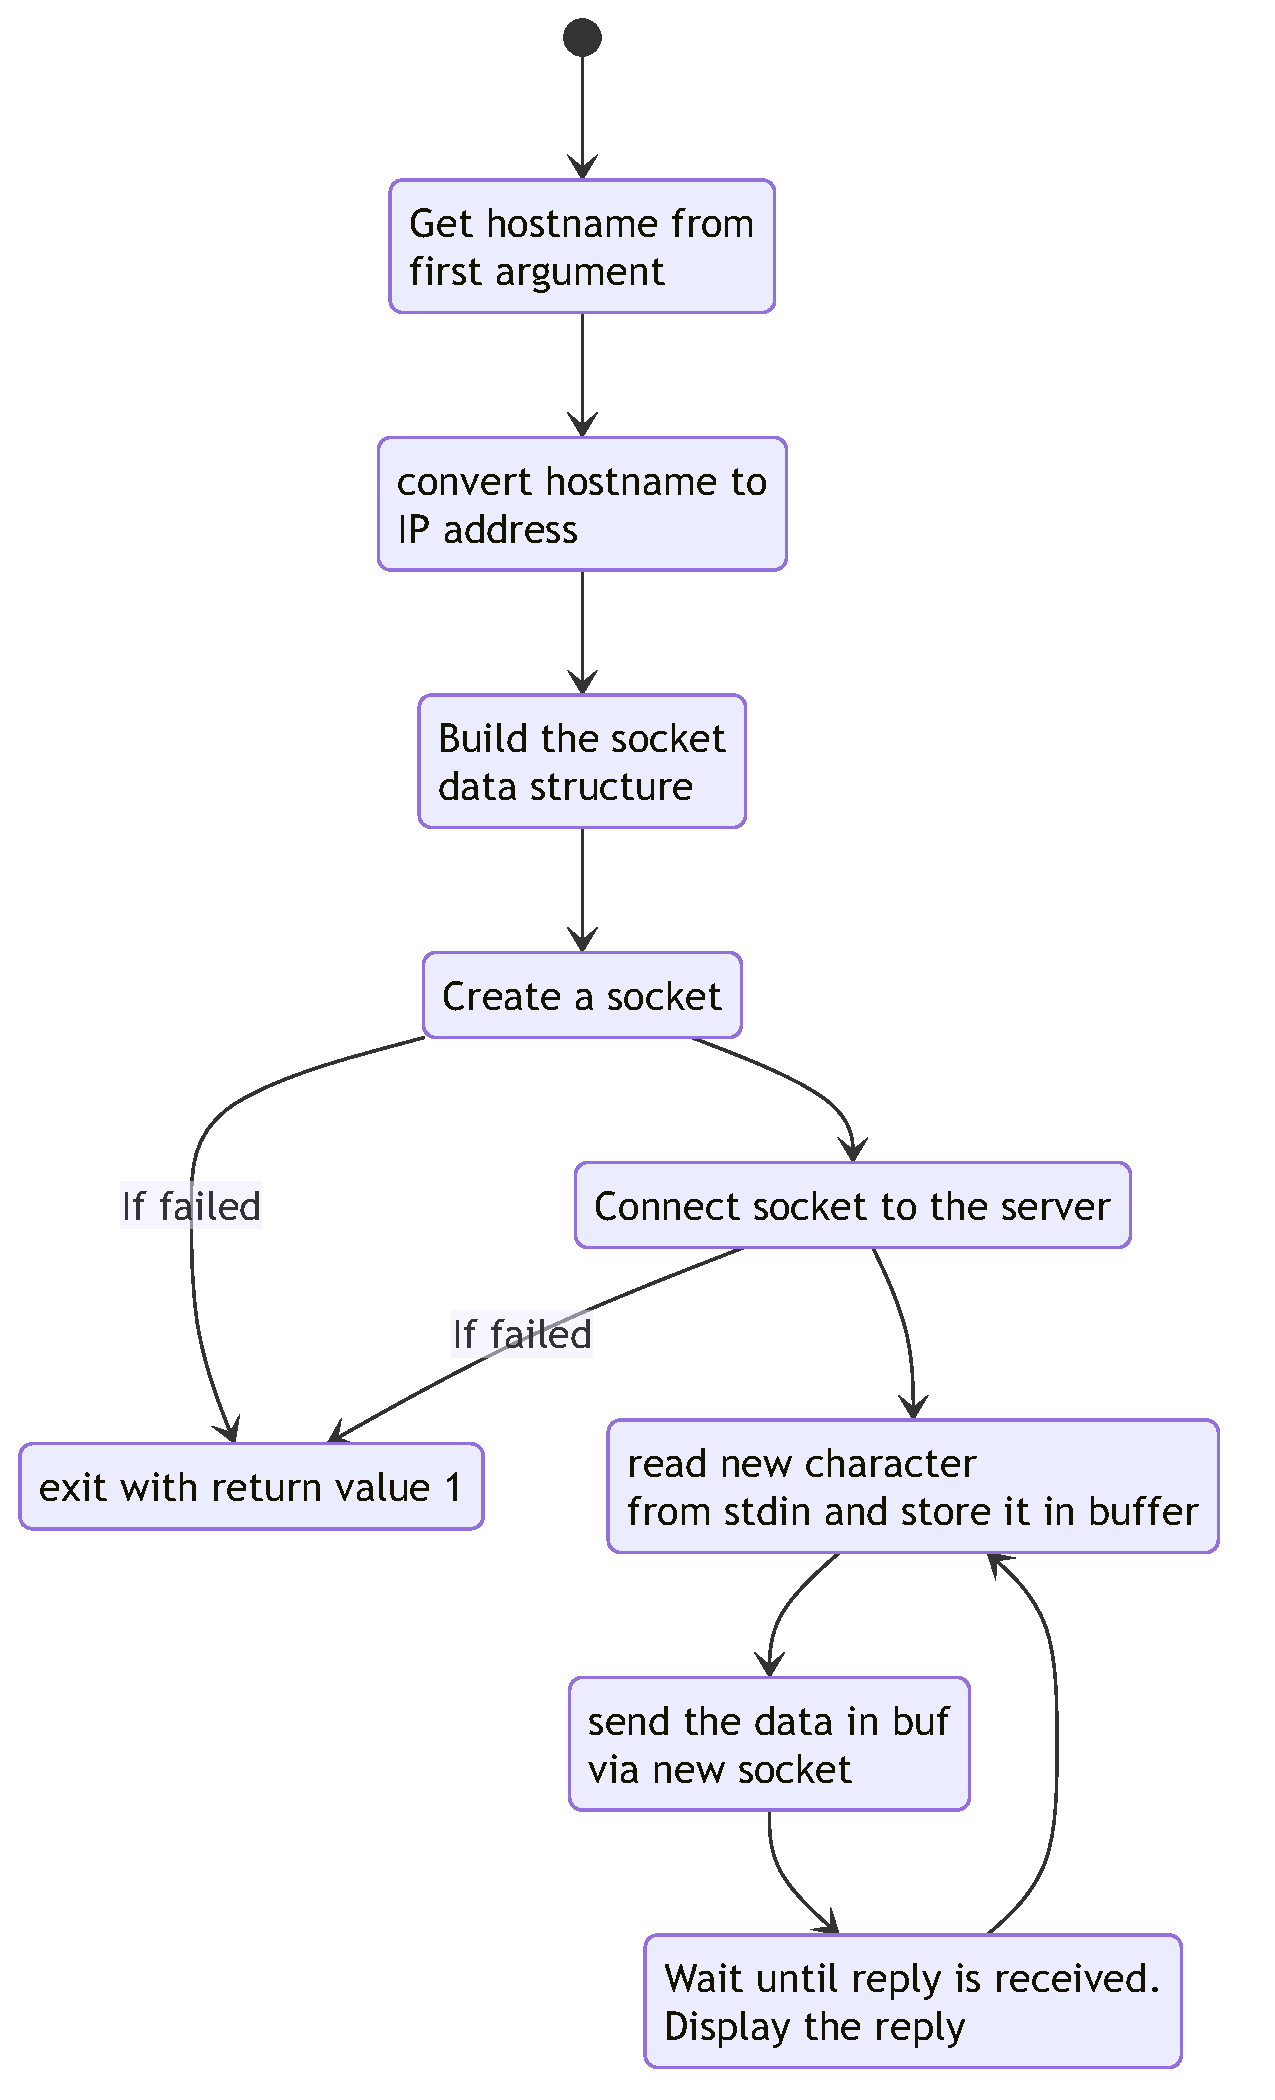
\includegraphics[width=0.9\linewidth]{client-side.pdf}
    \caption{Client Side}
\end{figure}


\newpage
\section{Code Section}

\vspace{5mm}
\subsection{Example 1}

\begin{lstlisting}
#include <stdio.h>
#include <stdlib.h>
#include <time.h>

int main() {
    srand(time(NULL)); // Seed the random number generator

    int randomNumber = rand() % 100 + 1; // Generate a random number between 1 and 100

    printf("Random number: %d\n", randomNumber);

    return 0;
}

\end{lstlisting}

\section{Outputs}

\begin{figure}[H]
    \centering
    
\includegraphics[width=0.8\linewidth]{great-output-great.jpg}
    \caption{Great output - Copied from the internet}
    
\end{figure}

\textbf{Image description - }Great output - Copied from the internet

\vspace{10mm}
\line(1,0){500}
\vspace{10mm}\\    
\large{\textbf{REFERENCES USED}}
 \begin{enumerate}
     \item Overleaf docs
     \item Random netizens.
 \end{enumerate}


\end{document}

